%!TEX root = ../Thesis.tex
\section{Balanced Scorecard (Patrick Künzl)}
\subsection{Definition}
Die Balance Scorecard ist eines von vielen Instrumenten, um eine zielführende
Komposition der Unternehmensthemen \glqq Strategiefindung\grqq~und
\glqq Strategieumsetzung\grqq~zu erreichen. \glqq In ihrem Konzept werden die
traditionellen finanziellen Kennzahlen durch eine Kunden-, eine 
interne Prozess- und eine Lern- und Entwicklungsperspektive
ergänzt.\glqq\footnote{siehe \cite{BalanceGabler}} \\
Die Balance Scorecard wurde in den 90er-Jahren von R.S. Kaplan und D.P. Norton
entwickelt und war das Resultat einer Studie unter zwölf amerikanischen
Unternehmen. Ziel der Studie war es, die damalig vorhandenen Kennzahlensysteme
an den neuzeitigen Anforderungen der Unternehmen anzupassen. \footnote{Vgl.
\cite{BalanceGabler}}
\subsection{Aufbau der Balance Scorecard}
\begin{figure}[H]
\centering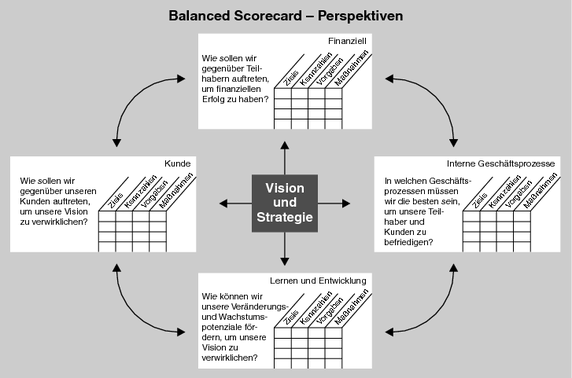
\includegraphics[width=1\textwidth]{img/bsc}
\caption[Aufbau einer Balance Scorecard]{schematische Darstellung des Aufbaus
einer Balance Scorecard - Quelle:
http://wirtschaftslexikon.gabler.de/Definition/balanced-scorecard.html,
Stand 03.04.2016}
\end{figure}
Die Balance Scorecard betrachtet das Unternehmen durch vier unterschiedliche
Perspektiven, welche nachfolgend kurz umschrieben werden:
\begin{itemize}
  \item finanzielle Sichtweise: \\
  Die finanzielle Sichtweise ist die älteste Perspektive des Modells. Dies kommt
  dadurch, dass die Basismodelle des Unternehmenscontrollings in den 50er Jahre
  die finanziellen Kennzahlen größtenteils als die einzig verlässlichen
  Parameter für den Erfolg eines Unternehmens lieferten. Die zentrale Frage, welche die
  finanzielle Perspektive beantworten möchte, lautet: \glqq Haben unsere getroffenen
  Maßnahmen und Strategien einen erfolgreichen Einfluss auf unseren
  Unternehmenserfolg?\glqq
  \item interne Geschäftsprozesse: \\
  Die Sicht der internen Geschäftsprozesse bietet die Möglichkeit Kennzahlen
  für, z. B. Durchlaufzeiten von verschiedenen Prozessen oder andere
  geschäftskritischen Workflows, zu analysieren und zu steuern. Ziel der Analyse
  der internen Prozesse beantwortet die Frage: \glqq In welchen Geschäftsprozessen
  müssen wir die besten sein, um unsere Teilhaber und Kunden zu befriedigen?\glqq
  \footnote{Vgl. mit obiger Abbildung}
  \item Lern- und Wachstumsperspektive: \\
  Die Lern- und Wachstumsperspektive ist die wichtigste Perspektive der gesamten
  Balanced Scorecard und bildet somit die Basis. Denn mit der Betrachtung der
  Mitarbeiter und den \glqq sozialen Faktoren\grqq~können erst alle anderen Ziele in 
  den anderen erreicht werden. \glqq Drei Hauptkategorien werden hierbei
  unterschieden: Qualifizierung von Mitarbeitern, Leistungsfähigkeit des 
  Informationssystems sowie Motivation und Zielausrichtung von Mitarbeitern.\glqq
  \footnote{siehe \cite{BalanceGabler}}
  \item Kundenperspektive: \\
  Die Kundenperspektive kümmert sich um jegliche Kennzahlen, die sich um den
  Kunden drehen. Es ist hierbei jedoch nicht zwingend notwendig, dass es externe
  Kunden sein müssen, sondern auch firmeninterne Abteilungen können Kunden für
  eine Abteilung sein, z. B. für die IT.
\end{itemize}
Wie man anhand der obigen Abbildung erkennen kann, stehen alle Perspektiven in
einer engen Beziehung zueinander, einer sogenannten
\glqq Ursache-Wirkung-Beziehung\glqq. Dies bedeutet, dass jegliche Anpassungen in einer
Perspektive ebenso Änderungen in anderen Perspektiven und den damit verbundenden
Kennzahlen mit sich bringt.
\subsection{Design der Balanced Scorecard für das Unternehmen Stylez}
Nachfolgend wird eine Strategie für das Unternehmen Stylez dargelegt. Dabei wird
jede Perspektive einzeln betrachtet und ausführlich dargestellt.
\subsubsection{finanzielle Perspektive}
\emph{Strategisches Ziel:} Um die eigene Marktposition weiter auszubauen, soll
die Anzahl der Franchise-Filialen weiterhin stark ansteigen\\
\emph{Kennzahl/Messgröße:} Anzahl der Franchise-Filialen\\
\emph{Zielwert:} 6 neue Filialen pro Jahr \\
\emph{Erforderliche Maßnahmen:} Durchführung einer guten Marketing-Strategie,
stetiger Ausbau des Bekanntheitsgrades, das Führen von Franchise-Filialen
attraktiver gestalten\\\\
\emph{Strategisches Ziel:} Erhöhung der Umsatzrendite im Online-Geschäft\\
\emph{Kennzahl/Messgröße:} Umsatzrendite des Online-Shops\\
\emph{Zielwert:} Steigerung um 3 Prozent \\
\emph{Erforderliche Maßnahmen:} Optimierung der IT-Infrastruktur, Verhandeln
von besseren Lieferantenkonditionen, Erhöhung der Gewinnspanne
\subsubsection{Kundenperspektive}
\emph{Strategisches Ziel:} Durch Anreizsysteme sollen Bestandskunden öfters
Neukunden werben\\
\emph{Kennzahl/Messgröße:} Neukunden pro Monat\\
\emph{Zielwert:} 25 Neukunden pro Monat \\
\emph{Erforderliche Maßnahmen:} Entwicklung eines Anreizsystems durch
Einführung eines Rabattsystems\\\\
\emph{Strategisches Ziel:} interne Abteilungen sollen zufriedener mit der
IT-Abteilung werden\\
\emph{Kennzahl/Messgröße:} Zufriedenheitsgrad der Mitarbeiter\\
\emph{Zielwert:} mindestens 4 von 5 Sternen \\
\emph{Erforderliche Maßnahmen:} Optimierung der IT-Infrastruktur, Mitarbeiter in
den Abteilungen schulen um kleinere Probleme selbst zu lösen, Einführung eines
Ticketsystem und Vorpriorisierung der Aufgaben für die IT-Mitarbeiter
\subsubsection{interne Prozessperspektive}
\emph{Strategisches Ziel:} benötigte Unternehmensdaten sollen den
Franchise-Filialen schneller zur Verfügung stehen\\
\emph{Kennzahl/Messgröße:} Geschwindigkeit der Datenabfrage und Transport in die
Filiale\\
\emph{Zielwert:} unter 5 Sekunden um jede Information zu bekommen \\
\emph{Erforderliche Maßnahmen:} Optimierung der Verbindungsleitungen,
Optimierung der IT-Infrastruktur, Fokus auf Hochverfügbarkeit von Daten
setzen\\\\
\emph{Strategisches Ziel:} Verkürzung der Wartungsarbeiten für IT-Mitarbeiter\\
\emph{Kennzahl/Messgröße:} Dauer der Wartungsarbeit\\
\emph{Zielwert:} pro Server im Haus nicht länger als 10 Minuten \\
\emph{Erforderliche Maßnahmen:} Optimierung der IT-Infrastruktur, Auslagerung
von Unternehmenssystemen nach Drittanbietern
\subsubsection{Lern- und Entwicklungsperspektive}
\emph{Strategisches Ziel:} Probleme bestehen in jeder Firma. Um die
Mitarbeiter an der Optimierung des Unternehmens teilhaben zu lassen, wird ein
betriebliches Verbesserungssystem eingeführt. Die Mitarbeiter sollen jedoch
selbst entscheiden, ob sie dran teilnehmen oder nicht.\\
\emph{Kennzahl/Messgröße:} Anzahl der Verbesserungsvorschläge pro Monat\\
\emph{Zielwert:} 3 pro Mitarbeiter pro Monat \\
\emph{Erforderliche Maßnahmen:} Einführung des betrieblichen
Vorschlagwesens, Einarbeitung der Mitarbeiter durch ein Anreizsystem bei
Durchführung\\\\
\emph{Strategisches Ziel:} konsequente Weiterbildung aller Mitarbeiter\\
\emph{Kennzahl/Messgröße:} Anzahl der Weiterbildungstage\\
\emph{Zielwert:} Mindestens 5 Tage pro Jahr \\
\emph{Erforderliche Maßnahmen:} Erweiterung des Schulungsangebots, Versand von
E-Mails mit externen Weiterbildungsmöglichkeiten, Einrichtung einer zentralen
Stelle zur Annahme von individuellen Weiterbildungsanfragen
\section{IT-Infrastruktur (Patrick Künzl)}
\label{sec:IT-Infrastruktur}
\subsection{Einleitende Worte}
Rückblickend auf die Balanced Scorecard erkennt man, dass viele Maßnahmen zur
Zielerreichung sich auf die Optimierung der IT-Infrastruktur stützen. Dies hat
in einem Unternehmen, welches sein Gewinn ausschließlich mit einem
Online-Geschäft und seiner Bereitstellung von Unternehmensdaten an nationale
Filialen erwirtschaftet, durchaus seine Berechtigung. Um diesen Gewinn nicht zu
gefährden, muss die IT-Strategie perfekt auf die Unternehmensstrategie angepasst
sein und muss die Anforderungen zur vollsten Zufriedenheit erfüllen.
Beispielhafte Anforderungen für die Zukunft wären:
\begin{itemize}
  \item Wahrung der Verfügbarkeit von Daten ohne Rücksicht auf Anzahl der
  eintreffenden Anfragen
  \item Wahrung eines optimalen Preis-/Leistungs-Verhältnisses
  \item Sicherung des Unternehmenserfolges
  \item Sicherung des Umsatzes
\end{itemize}
Die IT-Strategie versucht nun durch\ldots
\begin{itemize}
  \item \ldots eine leichte Skalierbarkeit der Hardware
  \item \ldots Verteilung der Auslastung und Abfangen von Belastungsspitzen
  \item \ldots Optimierung des Kostenspiegels
\end{itemize}
die Unternehmensstrategie erfolgreich zu unterstützen. Die Basis bildet dafür
die \glqq Grundhardware\glqq, die das Rückgrat der Unternehmens-IT bildet.
\subsection{Grundgedanke}
Start-Ups haben eine schwierige Ausgangssituation die interne IT zu optimieren.
Durch die fehlende Sicherung eines Wettbewerbsplatzes und der schwierigen
Abschätzbarkeit der notwendigen Ressourcen bei gleichzeitiger optimalen
Kostenkontrolle muss ein besonderes Augenmerk auf die Auslastung der Server
gelegt werden, da diese der Kostentreiber der IT sein können. Hier darf kein
Potenzial verschenkt werden. Daher wird der Vorschlag getätigt, die bisherigen
Server in der Unternehmenszentrale als Datenbankserver des Unternehmens
einzusetzen und Softwaresysteme mittels Infrastructure-as-a-Service
bereitzustellen, die wiederum per Direktleitung mit der Datenbank kommunizieren.
\subsubsection{Infrastructure-as-a-Service}
Bei Infrastructure-as-a-Service handelt sich um eins von vielen möglichen
Cloud-Modellen. Die Vorteile solch eines IT-Modells sind vielfältig: 
\begin{itemize}
  \item Kostenvorteile durch bedarfsgerechte Anpassung
  \item vorkonfektionierte Umgebungen mit modernster Technologie und sicherer
  Plattform
  \item keine Aufwände für Upgrades, Betrieb und Wartung
  \item Belastungsspitzen werden besser aufgefangen
  \item schnelle Skalierung des Systems auf die Echtzeit-Anforderungen
\end{itemize}
Datenschutzrichtlinien, Verbindungssicherheit und hohe Verfügbarkeit machen
Infrastructure-as-a-Service zu einem sehr attraktiven Gesamtpaket für junge
Unternehmen, die noch in der Aufbau- bzw. Expansionsphase sind. \\
Um dennoch weiterhin die Hoheitsrechte über die Unternehmensdaten zu wahren und
im extremsten Fall direkt und zu 100 Prozent über alle Daten zu verfügen, wird
die bisher bestehende Hardware in einen reinen Datenbankserver umgewandelt. Dieser
Datenbankserver gilt als zentrale Anlaufstelle für jegliche Software und ist per
direkter Leitung an die Cloud-Systeme der Anbieter angebunden, um eine schnelle
Übermittlung der Bytes zu gewährleisten.
\subsection{Amazon Web Services - Beispielrechnung}
\label{sec: AWS_Rechnung}
Um zu zeigen, dass es sich durchaus lohnt das IaaS-Konzept in die
Unternehmensstruktur aufzunehmen, anstatt die einzelnen Komponenten selbst zu
betreiben, betrachten wir die Gesamtkosten (Total Cost of Ownership) von einem
selbst-gekauften Server und einem angemieteten IaaS-Server.
\\ \\
\emph{Kostenaufstellung: eigener Server - Laufzeit 5 Jahre}
\begin{itemize}
  \item Anschaffungskosten:
  	\begin{itemize}
  	  \item Hardware: 2650\euro
  	  \item Betriebssystem (Server 2012 + CALs): 10000\euro
  	  \item Installationskosten: 1 MA, 8 Stunden für 110\euro/Stunde = 880\euro
  	\end{itemize}
  \item Betriebskosten:
  	\begin{itemize}
  	  \item Strom: 20\euro * 12 Monate * 5 Jahre = 1200\euro
  	  \item Wartung des Servers: 1 MA, 4 Stunden für 110\euro/Stunde, 1x pro
  	  Monat = 26400\euro
  	  \item Kosten für Ersatzteile: 1000\euro
  	\end{itemize}
  \item Entsorgungskosten:
  	\begin{itemize}
  	  \item Entsorgung: 100\euro
  	  \item Mitarbeiteraufwand: 1 MA, 4 Stunden für 110\euro/Stunde = 550\euro
  	\end{itemize}
  \item Gesamtsumme: 42780\euro
\end{itemize}
\underline{Kostenaufstellung: EC2 Server auf Amazon Web Services - Laufzeit 5
Jahre\footnote{die Preisangaben beziehen sich auf ein offizielles Whitepaper
von Amazon und sind dort in Dollar angegeben, Umrechnungskurs zum Euro: 1 US
Dollar = 0,87769\euro}}
\begin{itemize}
  \item Anschaffungskosten:
  	\begin{itemize}
  	  \item Hardware: 0\euro
  	  \item Betriebssystem (Server 2012 + CALs): 0\euro
  	  \item Installationskosten: 1 MA, 1 Stunde für 110\euro/Stunde = 110\euro
  	\end{itemize}
  \item Betriebskosten:
  	\begin{itemize}
  	  \item Strom: 20\euro * 12 Monate * 5 Jahre = 0\euro
  	  \item Wartung des Servers: 1 MA, 4 Stunden pro Jahr für 110\euro/Stunde =
  	  550\euro
  	  \item Kosten für Ersatzteile: 0\euro
  	  \item Amazon EC2 Instance Cost: Kosten pro Stunde 0,0614383\euro, 2
  	  Instanzen, 732 Stunden pro Monat = 5396,74\euro
  	  \item Elastic Load Balancer Cost: 732 Stunden pro Monat, Stundensatz von
  	  0,02194225\euro, Verarbeitete Daten [GB] 3000, Verarbeitungssatz von
  	  0,00702152\euro = 2227,58\euro
  	  \item AWS Data Transfer Cost: Empfangene Daten [GB] 2700 für 0,00\euro,
  	  Gesendete Daten [GB] 4100 für 0,1053228\euro = 25909,41\euro
  	\end{itemize}
  \item Entsorgungskosten:
  	\begin{itemize}
  	  \item Entsorgung: 0\euro
  	  \item Mitarbeiteraufwand: 1 MA, 1 Stunden für 110\euro/Stunde = 110\euro
  	\end{itemize}
  \item Gesamtsumme: 34303,73\euro
  \item Ersparnis gegenüber Self-Hosting-Variante: 8476,27\euro
\end{itemize}
Hier ist deutlich erkennbar, dass die Verwendung einer
Infrastructure-as-a-Service Lösung enorme Sparpotenziale hervorbringen kann.
Besonders durch die gesunkenen Aufwände für Wartung und die Verwendung dieser
gewonnenen Arbeitszeiten in andere Projekte, können die finanziellen
Strategieziele des Unternehmens optimal unterstützt werden.
